\documentclass[tikz, preview]{standalone}

\usepackage{tikz}
\usepackage[all,2cell]{xy}
\usetikzlibrary{matrix,arrows,shapes,decorations.markings,decorations.pathreplacing}
\definecolor{rewritecolor}{rgb}{0,.9,1}
\tikzset{rewritenode/.style={shape=circle,fill=rewritecolor,scale=0.25,font=\Huge}}
\tikzset{RWopen/.style={shape=circle,draw=black,fill=white,scale=0.5,font=\Huge}}
\tikzset{RWclosed/.style={shape=circle,fill=black,scale=0.5,font=\Huge}}
\tikzset{CDnode/.style={shape=circle,fill=white,scale=.5}}
\tikzset{zxgreen/.style={shape=circle,draw,thick,fill=green}}
\tikzset{zxred/.style={shape=circle,draw,thick,fill=red}}
\tikzset{zxyellow/.style={shape=rectangle,draw,thick,fill=yellow}}
\tikzset{zxdiamond/.style={shape=diamond,fill=black,inner sep=2.75pt}}
\tikzset{->-/.style={decoration={markings,mark=at position .5 with {\arrow{>}}},postaction={decorate}}}

\begin{document}
\[
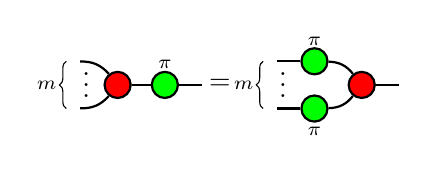
\begin{tikzpicture}
	\node (v2) at (0,0) {$=$};
	%
	%
	%
	\begin{scope}[shift={(0.2,0)}]
	\node [zxred] (v1) at (-1.5,0) {};
	\node (v3) at (-2.1,0.3) {};
	\node (v4) at (-2.1,-0.3) {};
	\node [zxgreen,label={[shift={(0,-0.1)}]\scriptsize $\pi$}] (v5) at (-0.9,0) {};
	\node (v6) at (-0.3,0) {};
	\node at (-1.9,0.1) {$\vdots$};
	\draw  (v1) edge[thick,bend right=25] (v3);
	\draw  (v1) edge[thick,bend left=25] (v4);
	\draw  (v1) edge[thick] (v5);
	\draw  (v5) edge[thick] (v6);
	\draw[decoration={brace,mirror,raise=5pt},decorate]
		(v3.east) -- node[left=5pt] {\scriptsize $m$} (v4.east); 
	\end{scope}
	%
	%
	%
	\begin{scope}[shift={(0.3,0)}]
	\node (v7) at (0.3,0.3) {};
	\node [zxgreen,label={[shift={(0,-0.1)}]\scriptsize $\pi$}] (v8) at (0.9,0.3) {};
	\node (v9) at (0.3,-0.3) {};
	\node [zxgreen,label={[shift={(0,-0.65)}]\scriptsize $\pi$}] (v10) at (0.9,-0.3) {};
	\node [zxred] (v11) at (1.5,0) {};
	\node (v12) at (2.1,0) {};
	\node at (0.5,0.1) {$\vdots$};
	%
	\draw  (v7) edge [thick] (v8);
	\draw  (v9) edge [thick] (v10);
	\draw  (v8) edge [thick,bend left=25] (v11);
	\draw  (v10) edge [thick,bend right=25] (v11);
	\draw  (v11) edge [thick] (v12);
	\draw[decoration={brace,mirror,raise=5pt},decorate]
		(v7.east) -- node[left=5pt] {\scriptsize $m$} (v9.east); 
	\end{scope}
\end{tikzpicture}
\]



\end{document}
